\chapter{Описание существующих решений}

В данном разделе представлено краткое описание существующих методов анализа
тональности естественно-языковых текстов.

\section{Лингвистический подход}

Методы использующие лингвистический подход можно разделить на две основные
категории:
\begin{itemize}
    \item методы на основе правил;
    \item методы на основе лексики.
\end{itemize}

Последние, в свою очередь, основываются либо на словарях слов, либо на корпусах
текстов.

\subsection{Методы, основанные на правилах}

\textit{Методы, основанные на правилах,} (или \textit{rule-based methods}) для
определения класса используют большой набор созданных в ручную правил
вида <<если $\rightarrow$ то>>~\cite{article14}. Левая часть каждого правила
показывает набор признаков, а правая часть --- метку класса~\cite{article2}.

В случае анализа тональности набор признаков может быть представлен словом,
словосочетанием или другой более сложной языковой конструкцией, а каждый класс
--- обозначен необходимым образом, например, символ <<$+$>>\ --- положительный,
<<$-$>> --- отрицательный. В таком случае одними из простейших
правил могут быть следующие (формулы \ref{eq:01}-\ref{eq:02}):
\begin{eqnarray}
    \{\text{хороший}\} \rightarrow \{+\}\label{eq:01}\\
    \{\text{плохой}\} \rightarrow \{-\}\label{eq:02}
\end{eqnarray}

Большой набор правил описанного вида позволяет осуществлять
прогнозирования тональности анализируемого текста~\cite{article16}.

Данные алгоритмы имеют отличную производительность в узких
областях тем текстов, однако их обобщение на более широкий круг тем
затруднительно. Также процесс создания необходимых правил является
трудоемким за счет их определения человеком, а не компьютером~\cite{article15}.

В целях ускорения процесса разработки для создания набора правил может
использоваться машинное обучение, поэтому в некоторых научных работах
\cite{article16}~\cite{article17} данные методы относят к методам машинного
обучения.

\subsection{Методы, основанные на тональных словарях}

\textit{Методы, основанные на тональных словарях,} (или \textit{dictionary-based
methods}) относят к методам, основанным на лексике.

В данном подходе вручную собирается небольшой набор уникальных слов и
словосочетаний, важных для тематики анализируемых текстов, с их тональными
оценками (весами)~\cite{article05}. Полученный набор увеличивается путем поиска в
онлайн-словарях синонимов и антонимов к каждому элементу, входящему в набор.
Найденные слова и словосочетания добавляются в исходный набор, и операция
повторяется до тех пор, пока при очередном повторении не будет получено ни
одного нового элемента набора~\cite{article4}. Итоговый набор, полученный
описанным методом, образует тональный словарь.

При анализе текста в итоговом наборе осуществляется поиск каждого слова и выбор
его веса. Если слова нет в словаре, то считают, что оно нейтрально, и
присваивают ему вес, равный нулю. По найденным весам высчитывается
принадлежности анализируемого текста к тому или иному классу
тональности~\cite{article05}.

Данный подход показывает хорошие результаты для некоторых областей, но
имеет плохую масштабируемость, то есть полученный в результате поиска
синонимов и антонимов словарь может быть корректно использован только для
той предметной области, для которой он составлялся. При этом выделение
начального небольшого набора слов и словосочетаний требует хороших
знаний в анализируемой предметной области, а следовательно, возникает
необходимость в изучении данной области или поиске специалиста, что приводит к
дополнительным трудозатратам~\cite{article05}.


\subsection{Методы, основанные на корпусах}

\textit{Методы, основанные на корпусах,} (или \textit{corpus-based
methods}) также относят к методам, основанным на лексике.

Данный подход так же, как и предыдущий, начинает работу с небольшого набора
слов, однако, в отличие от методов, основанных на тональных словарях, методы,
основанные на корпусах, осуществляют поиск слов для расширения исходного списка
в большом наборе анализируемых текстов, а не в онлайн-словарях~\cite{article2}.
Таким образом учитывается не только самостоятельная тональная оценка слова, но и
контекст, в котором это слово находится. При этом существует
два способа для учета контекста~\cite{article16}:
\begin{itemize}
    \item статистический подход учитывает число появлений слова в положительных
        и отрицательных текстах, при преобладании в первых считается, что
        тональная оценка слова положительна, при преобладании во вторых ---
        отрицательна, при совпадении частоты появлений --- нейтральна; при этом
        учитывается тот факт, что два слова часто встречающиеся вместе в одном
        контексте с высокой вероятностью будут иметь одинаковую
        \textbf{полярность}~\cite{article20};
    \item семантический подход опирается на различные принципы вычисления
        сходства между словами и присваивает словам близким по смыслу одинаковые
        значения веса~\cite{article20}.
\end{itemize}

Достоинством этого подхода является рассмотрение слова ни как самостоятельной
единицы с фиксированным весом, а как части единого текста с тональной оценкой,
зависящей от окружения~\cite{article2}; однако, так же как и в случае методов
на основе тональных словарей, список слов полученный для одного набора текстов
не может быть использован для анализа текстов иной предметной области, так как
одно и то же слово в различных областях может вносить разный вес эмоциональной
окраски~\cite{article05}.


\section{Методы машинного обучения}

В подходе к анализу тональности с точки зрения машинного обучения набор
текстов разделяется на две различные сборки: для обучающей и тестовой выборки.
Далее для контролируемого (с учителем) обучения тексты из обучающей
выборке размечаются, то есть указывается их класс тональности, а для
неконтролируемого (без учителя) обучения дополнительных данных не
указывается~\cite{article18}.

\subsection{Наивный байесовский классификатор}

\textit{Наивный байесовский классификатор}~\cite{article21} является
контролируемым вероятностным подходом, который определят тональность текста
путем нахождения наиболее вероятного класса $C_T$ для данного текста $T$, что
может быть описано формулой \ref{eq:03}:
\begin{equation}\label{eq:03}
    C_T = \argmax_C P(C|T),
\end{equation}

где $P(C|T)$ --- вероятность того, что текст $T$ принадлежит классу $C$,
которая может быть определена по формуле Баейса \ref{eq:04}.
\begin{equation}\label{eq:04}
    P(C|T) = \frac{P(C)P(T|C)}{P(T)},
\end{equation}

где $P(C)$ --- вероятность того, что встретится класс $C$ независимо от
анализируемого текста;

~~~~~~$P(T|C)$ --- вероятность встретить текст $T$ среди текстов класса $C$;

~~~~~~$P(T)$ --- вероятность того, что встретится текст $T$ среди всех текстов.

Вероятность $P(T)$ в формуле \ref{eq:04} не влияет на отношение текста к тому
или иному классу, поэтому может быть опущена.

При представлении текста в виде вектора входящих в него слов и предположении об
их независимости (что и дало данному классификатору название <<наивный>>)
вероятность встретить текст $T$ среди текстов класса $C$ может быть вычислена по
формуле \ref{eq:05}:
\begin{multline}\label{eq:05}
    P(T|C) = P(w_1, w_2, ..., w_N|C) = \\ =P(w_1|C) \cdot P(w_2|C) \cdot ...
    \cdot P(w_N|C) = \prod\limits_{i=1}^{N} P(w_i|C),
\end{multline}

где $w_i$ --- $i$-ое слово в тексте $T$;

~~~~~$P(w_i|C)$ --- вероятность встретить $i$-ое слово в классе $C$;

~~~~~$N$ --- количество слов в тексте.

Таким образом, с учетом формул \ref{eq:03}-\ref{eq:05} итоговый класс
анализируемого текста может быть найден по формуле \ref{eq:06}:

\begin{equation}\label{eq:06}
    C_T = \argmax_C P(C)P(T|C) = \argmax_C P(C)\prod\limits_{i=1}^{N} P(w_i|C).
\end{equation}

Наивный байесовский классификатор является самым простым и наиболее
используемым методом при решении задач с помощью машинного обучения,
однако данный метод делает предположение о независимости признаков (в случае
анализа тональности ими являются слова), которое в естественно-языковых текстах
обычно не подтверждается, что делает данный классификатор неэффективным.
Однако, несмотря на всю простоту и ограничение на независимость, наивный
байесовский классификатор может показывать хорошие результаты при анализе
тональности текста~\cite{article05}.

\subsection{Логическая регрессия}

\textit{Логическая регрессия} является методом линейного классификатора,
использующим для прогнозирования вероятности принадлежности текстов к классу
путем вычисления значения логической функции $f(z)$, описывающейся формулой
\ref{eq:07}:
\begin{equation}\label{eq:07}
    f(z) = \frac{1}{1+e^{-z}}.
\end{equation}

Параметр логической функции $z$ описывается формулой \ref{eq:08}:
\begin{equation}\label{eq:08}
    z = \theta^Tx=\theta_0+\theta_1x_1+...+\theta_nx_n,
\end{equation}

где $x$ --- вектор-столбец, в случае анализа тональности описывающий данный
текст;

$\theta$ --- вектор-столбец коэффициентов, получаемых в ходе обработке
обучающей выборки.

Для определения класса текста, он представляется в виде вектора столбца $x$,
далее вычисляется значение логической функции. Исходя из графика логической
функции, представленного на рисунке \ref{img:01}, если полученное значение
больше 0.5 текст считается положительным, иначе отрицательным~\cite{article22}.

\begin{figure}[h!]
    \begin{center}
        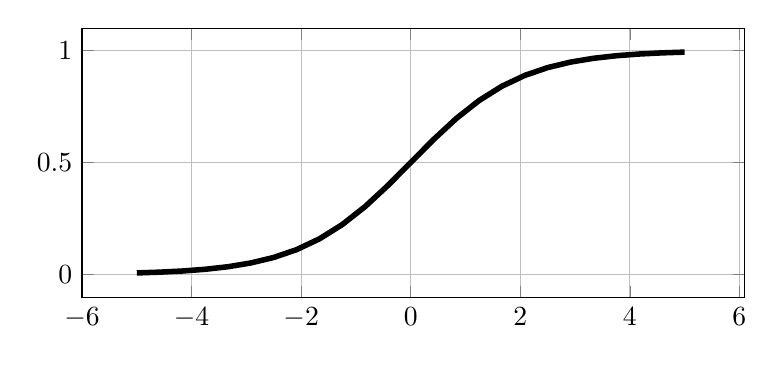
\begin{tikzpicture}
            \begin{axis} [
                width = 10cm,
                height = 5cm,
                xmin = -6,
                ymax = 1.1,
                grid = major
                ]
                \addplot[solid, line width = 2] {1 / (1 + e^(-x))};
            \end{axis}
        \end{tikzpicture}
    \end{center}
    \caption{График логической функции}\label{img:01}
\end{figure}

Логическая регрессия является одним из самых популярных методов классификации,
обученная модель показывает очень хорошие результаты, однако для работы
данного классификатора необходима качественная предобработка и отбор
признаков для представления текста в виде вектора-столбца~\cite{article05}.

\subsection{Метод максимума энтропии}

\textit{Метод максимума энтропии}~\cite{article23} является вероятностным
классификатором, который основан на принципе максимальной энтропии. По данному
принципу распределения вероятности являются равномерными (имеют максимальную
энтропию), если нет оснований считать иначе, то есть предположения о
независимости слов, как в случае наивного байесовского классификатора, не
делается, а при обучении максимизируются их веса с помощью итерационной
процедуры.

Вероятность $P(C|T)$ того, что текст $T$ принадлежит классу $C$, в данном случае
определяется формулой \ref{eq:09}:

\begin{equation}\label{eq:09}
    P(C|T) = \frac{1}{Z(T)}\exp\Big(\sum_i \lambda_i f_i(T, C)\Big),
\end{equation}

где $Z(T)$ --- коэффициент нормализации, гарантирующий выполнение условия
нормировки, вычисляющийся по формуле \ref{eq:10};

$\lambda_i$ --- вес $i$-ого признака;

$f_i(T, C)$ --- функция принадлежности $i$-ого признака текста $T$ классу
$C$.

\begin{equation}\label{eq:10}
    Z(T) = \sum_C\exp\Big(\sum_i \lambda_i f_i(T, C)\Big),
\end{equation}

где обозначения соответствуют обозначениям в формуле \ref{eq:09}.

В силу отсутствия предположения о независимости признаков как в
случае наивного байесовского классификатора метод максимума энтропии
позволяет добиться лучших результатов с сохранением простоты реализации и
необходимости для обучения малого числа данных~\cite{article05}.

\subsection{$k$-ближайших соседей}

\textit{$k$-ближайших соседей} --- метод, работа которого заключается в
поиске обучающих текстов, наиболее похожих на анализируемый, при этом построение
обучающих данных происходит с учетом соотношений текстов друг с другом.

Для определения тональности текста с помощью данного метода вычисляется
расстояние между тестовыми данными и уже обработанными обучающими. Чаще всего
для вычисления расстояния используют косинусное сходство (формула \ref{eq:11}),
соответствующее косинусу угла $\theta$ между векторами $\vec{A}$ и
$\vec{B}$, которые задают сравниваемые тексты.

\begin{equation}\label{eq:11}
    \cos{\theta} = \frac{\vec{A} \cdot \vec{B}}{\|\vec{A}\|\|\vec{B}\|} =
    \frac{\sum\limits_{i=1}^n{A_iB_i}}{\sqrt{\sum\limits_{i=1}^n{A_i^2}} \cdot
    \sqrt{\sum\limits_{i=1}^n{B_i^2}}}
\end{equation}

После вычисления всех расстояний в их наборе ищутся $k$ наименьших, при чем $k$
определяется заранее. И в конце анализируемому тексту сопоставляется тот класс,
к которому относится большинство из $k$ выбранных соседей.

Данный метод прост в реализации, однако имеет большое время выполнения в силу
необходимости полного перебора~\cite{article19}.

\subsection{Дерево решений}

Классификатор \textit{дерева решений} строит обучающие данные в древовидную
структуру: выбирается слово, тексты, которые его содержат, помещаются на правую
ветвь дерева, остальные --- в левую; для каждой ветви процедура повторяется до
тех пор, пока листья не будут содержать определенное минимальное количество
записей, которые используются для определения тональности. Таким образом,
внутренние узлы дерева представляют условие, являющееся проверкой на наличие
или отсутствие одного или нескольких слов, а листья содержат либо минимальный
набор текстов, по которым можно определить тональность анализируемого, либо
метку класса, к которому будет принадлежать текст, удовлетворяющий всем
условиям, включенным в путь от корня к данному листу.

При анализе тональности текста, не входящего в обучающую выборку, для него,
начиная с корня построенного дерева, проверяются условия во внутренних узлах для
поиска необходимого листа, по информации из которого определяется тональность
~\cite{article4}.

Метод дерева решений является рекурсивным, прост в реализации, требует
минимальной предварительной обработки данных и дает хорошие результаты при
решении задачи анализа тональности текста на большом количестве данных, однако
данный метод сильно зависит от обучающих данных, то есть при небольших
изменениях в обучающей выборке, получаются кардинально разные результаты на
тестовых данных~\cite{article05}.

\subsection{Случайный лес}

Для решения проблемы дерева решений с зависимостью от обучающих данных
используется ансамбль решающих деревьев, или \textit{случайный лес}.
В данном методе строится большое количество решающих деревьев на разных
обучающих данных по алгоритму, описанному в предыдущем пункте. Для определения
тональности текста, он анализируется с помощью каждого дерева, класс, выбранный
большинством деревьев, определяет тональность анализируемого текста.

Данный метод решает проблемы одиночного решающего дерева, однако требует больших
временных затрат на построение деревьев~\cite{article05}.

\subsection{Метод опорных векторов}

\textit{Метод опорных векторов} является контролируемым линейным подходом. При
решении задачи классификации текстов, в том числе на положительные и
отрицательные, тексты обучающей выборки представляются в виде векторов, которым
соответствуют точки в $n$-мерном пространстве, где $n$ --- размерность вектора.
Цель метода заключается в поиске такой гиперплоскости пространства, что сумма
расстояний от ближайших к этой гиперплоскости точек в каждом классе
(называющихся опорными векторами) максимальна (рисунок
\ref{img:02})~\cite{article16}.

\img{7cm}{svm}{Визуализация метода опорных векторов}{02}

Данный метод является одним из наиболее эффективных методов классификации
и показывает хорошие результаты при классификации текстов, так как
хорошо масштабируется и может работать с большим количеством признаков на
больших выборках~\cite{article05}.

\subsection{Нейронные сети}

\textit{Нейронные сети}~\cite{article05} являются математической моделью,
построенной по принципу организации и функционирования биологических нейронных
сетей. Основными трудностями при их использовании являются необходимость
большого количества обучающих данных, ресурсов и времени, а также  их настройка:
определение количества скрытых слоев, функции активации для каждого узла и
пороговой ошибки. Однако нейронные сети способны отбирать признаки без участия
человека, определять сложные зависимости между входными и выходными данными, а
также адаптироваться к изменениям, благодаря чему нейронные сети зарекомендовали
себя во многих областях, в том числе в анализе тональности текстов.

Наиболее распространенными нейронными сетями в области анализа тональности
текстов являются \textit{сверточные} и \textit{рекуррентные}. Сверточные
нейронные сети используют операцию свертки (текст разбивается на фрагменты,
каждый из которых умножается на матрицу свертки поэлементно, после чего результат
суммируется), которая происходит на соседних словах, что позволяет учесть
контекст, например, отрицания. Рекуррентные нейронные сети имеют  обратные связи
от более удаленных элементов к менее, что позволяет сети учитывать не только
текущие, но и предыдущие входные данные, благодаря чему вес каждого слова влияет
на веса остальных слов в предложении.

\section{Гибридные методы}

Для объединения преимуществ лингвистического похода и методов машинного обучения
разрабатываются \textit{гибридные методы}, сочетающие в себе два и более из описанных
методов~\cite{article5}. Так, для решения задачи анализа тональности были
объединены тональные словари и метод опорных векторов, сверточные нейронные сети
и k-ближайших соседей~\cite{article14}, также в одной из работ была разработана
гибридная система анализа тональности, объединившая методы на основе
правил и сверточную нейронную сеть.

Сочетание сильных сторон подходов на основе лингвистики и машинного обучения
позволяет получить более точные результаты, однако в то же время гибридные
методы получают проблемы и ограничения каждого из
подходов~\cite{article15}.

